\documentclass[twoside,11pt]{article}

% Any additional packages needed should be included after jmlr2e.
% Note that jmlr2e.sty includes epsfig, amssymb, natbib and graphicx,
% and defines many common macros, such as 'proof' and 'example'.
%
% It also sets the bibliographystyle to plainnat; for more information on
% natbib citation styles, see the natbib documentation, a copy of which
% is archived at http://www.jmlr.org/format/natbib.pdf

\usepackage{jmlr2e}
\usepackage{multirow}
\usepackage{booktabs}
\usepackage{xspace}
\usepackage[table]{xcolor}
\usepackage{graphicx}
\usepackage{subfig}
\usepackage[inline]{enumitem}
\usepackage{hyperref}
\usepackage{amsmath,amsfonts,dsfont,mathrsfs,mathtools,amssymb}
\usepackage{algorithm, algpseudocode}

\usepackage{fancyvrb}
\usepackage{color}
\usepackage[utf8]{inputenc}


\makeatletter
\def\PY@reset{\let\PY@it=\relax \let\PY@bf=\relax%
    \let\PY@ul=\relax \let\PY@tc=\relax%
    \let\PY@bc=\relax \let\PY@ff=\relax}
\def\PY@tok#1{\csname PY@tok@#1\endcsname}
\def\PY@toks#1+{\ifx\relax#1\empty\else%
    \PY@tok{#1}\expandafter\PY@toks\fi}
\def\PY@do#1{\PY@bc{\PY@tc{\PY@ul{%
    \PY@it{\PY@bf{\PY@ff{#1}}}}}}}
\def\PY#1#2{\PY@reset\PY@toks#1+\relax+\PY@do{#2}}

\expandafter\def\csname PY@tok@se\endcsname{\let\PY@bf=\textbf\def\PY@tc##1{\textcolor[rgb]{0.73,0.40,0.13}{##1}}}
\expandafter\def\csname PY@tok@kp\endcsname{\def\PY@tc##1{\textcolor[rgb]{0.67,0.13,1.00}{##1}}}
\expandafter\def\csname PY@tok@il\endcsname{\def\PY@tc##1{\textcolor[rgb]{0.40,0.40,0.40}{##1}}}
\expandafter\def\csname PY@tok@cm\endcsname{\let\PY@it=\textit\def\PY@tc##1{\textcolor[rgb]{0.00,0.53,0.00}{##1}}}
\expandafter\def\csname PY@tok@ow\endcsname{\let\PY@bf=\textbf\def\PY@tc##1{\textcolor[rgb]{0.67,0.13,1.00}{##1}}}
\expandafter\def\csname PY@tok@nn\endcsname{\let\PY@bf=\textbf\def\PY@tc##1{\textcolor[rgb]{0.00,0.00,1.00}{##1}}}
\expandafter\def\csname PY@tok@gd\endcsname{\def\PY@tc##1{\textcolor[rgb]{0.63,0.00,0.00}{##1}}}
\expandafter\def\csname PY@tok@kr\endcsname{\let\PY@bf=\textbf\def\PY@tc##1{\textcolor[rgb]{0.67,0.13,1.00}{##1}}}
\expandafter\def\csname PY@tok@cpf\endcsname{\let\PY@it=\textit\def\PY@tc##1{\textcolor[rgb]{0.00,0.53,0.00}{##1}}}
\expandafter\def\csname PY@tok@gt\endcsname{\def\PY@tc##1{\textcolor[rgb]{0.00,0.27,0.87}{##1}}}
\expandafter\def\csname PY@tok@gh\endcsname{\let\PY@bf=\textbf\def\PY@tc##1{\textcolor[rgb]{0.00,0.00,0.50}{##1}}}
\expandafter\def\csname PY@tok@c\endcsname{\let\PY@it=\textit\def\PY@tc##1{\textcolor[rgb]{0.00,0.53,0.00}{##1}}}
\expandafter\def\csname PY@tok@s2\endcsname{\def\PY@tc##1{\textcolor[rgb]{0.73,0.27,0.27}{##1}}}
\expandafter\def\csname PY@tok@gp\endcsname{\let\PY@bf=\textbf\def\PY@tc##1{\textcolor[rgb]{0.00,0.00,0.50}{##1}}}
\expandafter\def\csname PY@tok@ge\endcsname{\let\PY@it=\textit}
\expandafter\def\csname PY@tok@na\endcsname{\def\PY@tc##1{\textcolor[rgb]{0.73,0.27,0.27}{##1}}}
\expandafter\def\csname PY@tok@gi\endcsname{\def\PY@tc##1{\textcolor[rgb]{0.00,0.63,0.00}{##1}}}
\expandafter\def\csname PY@tok@mb\endcsname{\def\PY@tc##1{\textcolor[rgb]{0.40,0.40,0.40}{##1}}}
\expandafter\def\csname PY@tok@ch\endcsname{\let\PY@it=\textit\def\PY@tc##1{\textcolor[rgb]{0.00,0.53,0.00}{##1}}}
\expandafter\def\csname PY@tok@kc\endcsname{\let\PY@bf=\textbf\def\PY@tc##1{\textcolor[rgb]{0.67,0.13,1.00}{##1}}}
\expandafter\def\csname PY@tok@kd\endcsname{\let\PY@bf=\textbf\def\PY@tc##1{\textcolor[rgb]{0.67,0.13,1.00}{##1}}}
\expandafter\def\csname PY@tok@no\endcsname{\def\PY@tc##1{\textcolor[rgb]{0.53,0.00,0.00}{##1}}}
\expandafter\def\csname PY@tok@s\endcsname{\def\PY@tc##1{\textcolor[rgb]{0.73,0.27,0.27}{##1}}}
\expandafter\def\csname PY@tok@kn\endcsname{\let\PY@bf=\textbf\def\PY@tc##1{\textcolor[rgb]{0.67,0.13,1.00}{##1}}}
\expandafter\def\csname PY@tok@vg\endcsname{\def\PY@tc##1{\textcolor[rgb]{0.72,0.53,0.04}{##1}}}
\expandafter\def\csname PY@tok@vi\endcsname{\def\PY@tc##1{\textcolor[rgb]{0.72,0.53,0.04}{##1}}}
\expandafter\def\csname PY@tok@mo\endcsname{\def\PY@tc##1{\textcolor[rgb]{0.40,0.40,0.40}{##1}}}
\expandafter\def\csname PY@tok@sr\endcsname{\def\PY@tc##1{\textcolor[rgb]{0.73,0.40,0.53}{##1}}}
\expandafter\def\csname PY@tok@cs\endcsname{\let\PY@bf=\textbf\def\PY@tc##1{\textcolor[rgb]{0.00,0.53,0.00}{##1}}}
\expandafter\def\csname PY@tok@mh\endcsname{\def\PY@tc##1{\textcolor[rgb]{0.40,0.40,0.40}{##1}}}
\expandafter\def\csname PY@tok@ss\endcsname{\def\PY@tc##1{\textcolor[rgb]{0.72,0.53,0.04}{##1}}}
\expandafter\def\csname PY@tok@nb\endcsname{\def\PY@tc##1{\textcolor[rgb]{0.67,0.13,1.00}{##1}}}
\expandafter\def\csname PY@tok@sx\endcsname{\def\PY@tc##1{\textcolor[rgb]{0.00,0.50,0.00}{##1}}}
\expandafter\def\csname PY@tok@sb\endcsname{\def\PY@tc##1{\textcolor[rgb]{0.73,0.27,0.27}{##1}}}
\expandafter\def\csname PY@tok@mi\endcsname{\def\PY@tc##1{\textcolor[rgb]{0.40,0.40,0.40}{##1}}}
\expandafter\def\csname PY@tok@si\endcsname{\let\PY@bf=\textbf\def\PY@tc##1{\textcolor[rgb]{0.73,0.40,0.53}{##1}}}
\expandafter\def\csname PY@tok@s1\endcsname{\def\PY@tc##1{\textcolor[rgb]{0.73,0.27,0.27}{##1}}}
\expandafter\def\csname PY@tok@gu\endcsname{\let\PY@bf=\textbf\def\PY@tc##1{\textcolor[rgb]{0.50,0.00,0.50}{##1}}}
\expandafter\def\csname PY@tok@nt\endcsname{\let\PY@bf=\textbf\def\PY@tc##1{\textcolor[rgb]{0.00,0.50,0.00}{##1}}}
\expandafter\def\csname PY@tok@vc\endcsname{\def\PY@tc##1{\textcolor[rgb]{0.72,0.53,0.04}{##1}}}
\expandafter\def\csname PY@tok@ni\endcsname{\let\PY@bf=\textbf\def\PY@tc##1{\textcolor[rgb]{0.60,0.60,0.60}{##1}}}
\expandafter\def\csname PY@tok@sc\endcsname{\def\PY@tc##1{\textcolor[rgb]{0.73,0.27,0.27}{##1}}}
\expandafter\def\csname PY@tok@ne\endcsname{\let\PY@bf=\textbf\def\PY@tc##1{\textcolor[rgb]{0.82,0.25,0.23}{##1}}}
\expandafter\def\csname PY@tok@c1\endcsname{\let\PY@it=\textit\def\PY@tc##1{\textcolor[rgb]{0.00,0.53,0.00}{##1}}}
\expandafter\def\csname PY@tok@nc\endcsname{\def\PY@tc##1{\textcolor[rgb]{0.00,0.00,1.00}{##1}}}
\expandafter\def\csname PY@tok@nv\endcsname{\def\PY@tc##1{\textcolor[rgb]{0.72,0.53,0.04}{##1}}}
\expandafter\def\csname PY@tok@sh\endcsname{\def\PY@tc##1{\textcolor[rgb]{0.73,0.27,0.27}{##1}}}
\expandafter\def\csname PY@tok@bp\endcsname{\def\PY@tc##1{\textcolor[rgb]{0.67,0.13,1.00}{##1}}}
\expandafter\def\csname PY@tok@go\endcsname{\def\PY@tc##1{\textcolor[rgb]{0.53,0.53,0.53}{##1}}}
\expandafter\def\csname PY@tok@kt\endcsname{\let\PY@bf=\textbf\def\PY@tc##1{\textcolor[rgb]{0.00,0.73,0.00}{##1}}}
\expandafter\def\csname PY@tok@gs\endcsname{\let\PY@bf=\textbf}
\expandafter\def\csname PY@tok@nl\endcsname{\def\PY@tc##1{\textcolor[rgb]{0.63,0.63,0.00}{##1}}}
\expandafter\def\csname PY@tok@err\endcsname{\def\PY@bc##1{\setlength{\fboxsep}{0pt}\fcolorbox[rgb]{1.00,0.00,0.00}{1,1,1}{\strut ##1}}}
\expandafter\def\csname PY@tok@w\endcsname{\def\PY@tc##1{\textcolor[rgb]{0.73,0.73,0.73}{##1}}}
\expandafter\def\csname PY@tok@o\endcsname{\def\PY@tc##1{\textcolor[rgb]{0.40,0.40,0.40}{##1}}}
\expandafter\def\csname PY@tok@sd\endcsname{\let\PY@it=\textit\def\PY@tc##1{\textcolor[rgb]{0.73,0.27,0.27}{##1}}}
\expandafter\def\csname PY@tok@k\endcsname{\let\PY@bf=\textbf\def\PY@tc##1{\textcolor[rgb]{0.67,0.13,1.00}{##1}}}
\expandafter\def\csname PY@tok@gr\endcsname{\def\PY@tc##1{\textcolor[rgb]{1.00,0.00,0.00}{##1}}}
\expandafter\def\csname PY@tok@mf\endcsname{\def\PY@tc##1{\textcolor[rgb]{0.40,0.40,0.40}{##1}}}
\expandafter\def\csname PY@tok@cp\endcsname{\def\PY@tc##1{\textcolor[rgb]{0.00,0.53,0.00}{##1}}}
\expandafter\def\csname PY@tok@m\endcsname{\def\PY@tc##1{\textcolor[rgb]{0.40,0.40,0.40}{##1}}}
\expandafter\def\csname PY@tok@nd\endcsname{\def\PY@tc##1{\textcolor[rgb]{0.67,0.13,1.00}{##1}}}
\expandafter\def\csname PY@tok@nf\endcsname{\def\PY@tc##1{\textcolor[rgb]{0.00,0.63,0.00}{##1}}}

\def\PYZbs{\char`\\}
\def\PYZus{\char`\_}
\def\PYZob{\char`\{}
\def\PYZcb{\char`\}}
\def\PYZca{\char`\^}
\def\PYZam{\char`\&}
\def\PYZlt{\char`\<}
\def\PYZgt{\char`\>}
\def\PYZsh{\char`\#}
\def\PYZpc{\char`\%}
\def\PYZdl{\char`\$}
\def\PYZhy{\char`\-}
\def\PYZsq{\char`\'}
\def\PYZdq{\char`\"}
\def\PYZti{\char`\~}
% for compatibility with earlier versions
\def\PYZat{@}
\def\PYZlb{[}
\def\PYZrb{]}
\makeatother

\newcommand{\argmax}[1]{\underset{#1}{\operatorname{arg}\,\operatorname{max}}\;}
% \usepackage{showframe}

% Definitions of handy macros can go here
\newcommand{\dataset}{{\cal D}}
\newcommand{\fracpartial}[2]{\frac{\partial #1}{\partial  #2}}

\newcommand{\ade}{\texttt{Adenine}\@\xspace}
\newcommand{\py}{\texttt{Python}\@\xspace}
\newcommand*{\ie}{i.e.\@\xspace}
\newcommand*{\eg}{e.g.\@\xspace}
\newcommand{\todo}[1]{\textcolor{red}{{\bf \{#1\}}}} %TODO

% Heading arguments are {volume}{year}{pages}{submitted}{published}{author-full-names}
\jmlrheading{X}{2016}{X-XX}{X/XX}{XX/XX}{Samuele Fiorini, Federico Tomasi and Annalisa Barla}

% Short headings should be running head and authors last names

\ShortHeadings{ADENINE}{Fiorini, Tomasi, Barla}
\firstpageno{1}

\begin{document}

\title{ADENINE --- A Data ExploratioN pIpeliNE}

\author{\name{Samuele Fiorini} \email{samuele.fiorini@dibris.unige.it}\\
\name{Federico Tomasi} \email{federico.tomasi@dibris.unige.it}\\
\name{Annalisa Barla} \email{annalisa.barla@unige.it}\\[1em]
\addr Department of Informatics, Bioengineering, \\Robotics and System Engineering (DIBRIS)\\
     University of Genoa\\
     Genoa, I-16146, Italy}


\editor{Editor name}

\maketitle

\begin{abstract}

In this paper we introduce \ade, a machine learning \py framework for data exploration. The main goal of \ade{} is twofold: helping researchers and data scientists achieving a first and quick overview on the main structures underlying their data and choosing the most suitable unsupervised learning pipeline for the problem at hand. This software tool encompasses state-of-the-art techniques for: missing values imputing, data preprocessing, dimensionality reduction and clustering tasks.
\ade exploits both process- and thread-level parallelism and it is capable of generating nice and clean publication-ready plots along with quantitative descriptions of pipeline results. \ade is released under FreeBSD license and it can be downloaded from \href{http://slipguru.github.io/adenine/}{http://slipguru.github.io/adenine/}.
%% max 200 words: current ~100

\end{abstract}

\begin{keywords}
Data exploration, unsupervised learning, RNA-Seq gene expression
\end{keywords}

\section{Introduction}\label{sec:intro}
Data exploration is a very insightful starting point for many data analysis projects. Researchers and data scientists are often asked to extract meaningful information from collections of complex and possibly high-dimensional data coming from heterogeneous contexts. For instance, in biomedical scenarios, physicians are likely to be interested in answering some biological questions starting from observations collected from a pool of subjects enrolled in a study. Possible investigations can be: \emph{is there any relevant stratification among subjects?} or \emph{is it possible to discriminate between cases and controls from my observations?}. Starting from a given dataset, the information needed to answer such questions may be non-trivial to extract or even completely absent.
In these situations, a preliminary data exploration step is not only a good practice, but also a fundamental starting point for further and deeper investigations. To accomplish this task, several machine learning and data mining techniques were developed over the years. Among those we focus on the four most popular classes of methods: \begin{enumerate*}[label=(\roman*)]
  \item missing values imputing,
  \item data preprocessing,
  \item dimensionality reduction and
  \item unsupervised clustering
\end{enumerate*}.

In the last few years, a fair number of data exploration software and libraries were released. At a very coarse grain we can group them in two families: GUI-based and command-line applications. 
Among the first group we recall \emph{Divvy} \citep{lewis2013divvy}, a software tool that performs dimensionality reduction and clustering on input datasets. \emph{Divvy} is a light framework, with a Mac OS X designed interface. However,
%it heavily lacks in documentation, 
its collection of \texttt{C/C++} algorithm implementations does not cover common strategies such as kernel principal component analysis (KPCA) \citep{scholkopf1997kernel} or hierarchical clustering \citep{friedman2001elements} and it does not offer strategies to perform automatic discoveries of the number of clusters. The most notable project that spans between the two families is \emph{Orange} \citep{demvsar2013orange}, a data mining software suite that offers both visual programming front-end and \py APIs. In the context of data exploration, \emph{Orange} can be successfully employed. However, it does not support automatic pipeline generation, hence it requires the user to manually create each pipeline. Also, as of today \emph{Orange} lacks in several nonlinear methods such as isomap \citep{tenenbaum2000global}, locally linear embedding \citep{roweis2000nonlinear} and spectral clustering \citep{shi2000normalized}.

We introduce \ade, a command-line \py tool for data exploration that, starting from a set of unsupervised algorithms, creates textual an graphical reports of an arbitrary number of pipelines. In this context data imputing, preprocessing, dimensionality reduction and clustering strategies are considered as building blocks for data analysis pipelines. The user is only required to specify input data and to select blocks, then \ade takes care of the generation and running of the pipelines composed by all possible combinations of the selected algorithms. Every algorithm implementation of \ade is inherited, or extended, from \texttt{scikit-learn} \citep{scikit-learn} which is, to the best of our knowledge, the most complete machine learning open source library freely available online.

%%%%%%%%%%%%%%%%%%%%%%%%%%%%%%%%%%%%%%%%%%%%%%%%%%%%%%%%%%%%%%%%%%%%%%%%

\section{Tool overview}\label{sec:implem}
\ade is developed around the data analysis concept of \emph{pipeline}. A pipeline is a sequence of the following fundamental steps:
\begin{enumerate*}[label=(\roman*)]
  \item missing values imputing,
  \item data preprocessing,
  \item dimensionality reduction and
  \item unsupervised clustering
\end{enumerate*}. 
%(see Figure~\ref{fig:workflow}).
For each task, different off-the-shelf algorithms are available (see Table~\ref{tab:blocks}).%, however none of such steps are mandatory and they can be skipped if not required.

%\begin{figure}[h!]
%    \centering
%    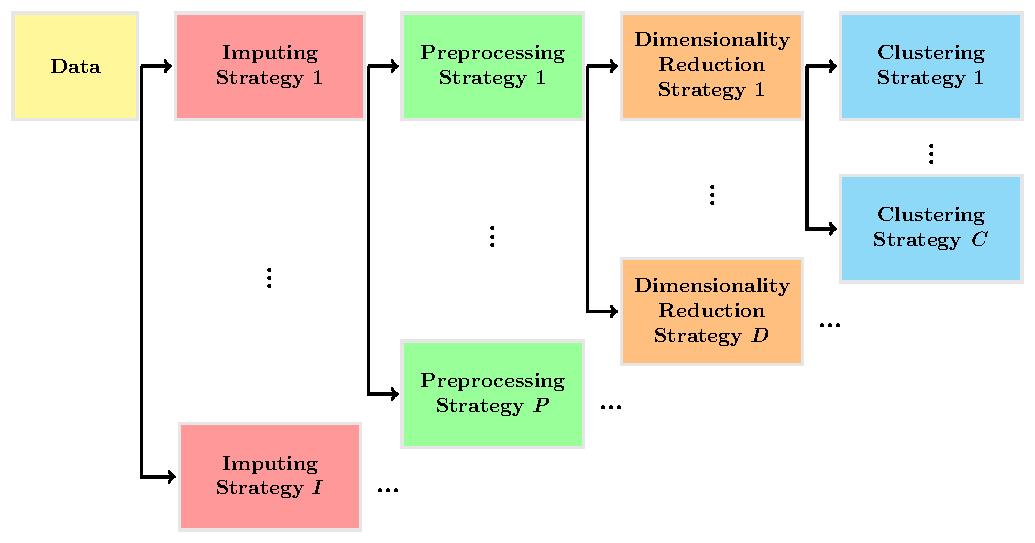
\includegraphics[width=\textwidth]{ade_wf/ade_wf.pdf}
%    \caption{A schematic representation of the \ade workflow. The list of building blocks available for each step is summarized in Table~\ref{tab:blocks}. The final number of pipelines generated is $I \times P \times D \times C$.}\label{fig:workflow}
%\end{figure}


    \begin{table}[]
    \small

    \centering

      \begin{tabular}{lll}
          \toprule
          \bfseries Step &   \bfseries Algorithm & \bfseries Reference\\

          \multirow{2}{*}{Imputing} & mean &  \\
          & median & \\
          & most frequent & \\
          & $k$-nearest neighbors & \citep{troyanskaya2001missing} \\
          \midrule

          \multirow{4}{*}{Preprocessing} & recentering &  \\
          & standardize &  \\
          & normalize &  \\
          & min-max &  \\
          \midrule

          \multirow{9}{*}{\begin{tabular}{@{}c@{}}Dimensionality \\ reduction\end{tabular}} & principal component analysis (PCA)& \citep{jolliffe2002principal} \\
          & incremental PCA & \citep{ross2008incremental} \\
          & randomized PCA & \citep{halko2011finding} \\
          & kernel PCA & \citep{scholkopf1997kernel} \\
          & isomap & \citep{tenenbaum2000global} \\
          & locally linear embedding & \citep{roweis2000nonlinear} \\
          & spectral embedding & \citep{ng2002spectral} \\
          & multidimensional scaling & \citep{borg2005modern} \\
          & \begin{tabular}{@{}l@{}}t-distributed stochastic \\ neighbor embedding \end{tabular}   & \citep{van2008visualizing} \\
          \midrule

          \multirow{5}{*}{Clustering} & k-means &  \citep{bishop2006pattern}\\
          & affinity propagation & \citep{frey2007clustering} \\
          & mean shift & \citep{comaniciu2002mean} \\
          & spectral & \citep{shi2000normalized} \\
          & hierarchical & \citep{friedman2001elements} \\

          \bottomrule
      \end{tabular}

      \caption{Pipeline building blocks available in \ade. See \ade documentation for a comprehensive description.}\label{tab:blocks}

\end{table}


%       Correspondent references  are not specified for methods defined Section~\ref{sec:implem}.


\begin{enumerate}[leftmargin=*]
\item[]{\bf Step 0: Missing values imputing.}
  % \subsection*{Missing values imputing}
  In order to cope with real-world datasets where entries are often missing, \ade offers an improved version of the Imputer class provided by \texttt{scikit-learn}. Our extension adds a k-nearest neighbor (KNN) imputing method to the pre-existent features-wise \emph{mean}, \emph{median} and \emph{most frequent} value strategies. \citep{troyanskaya2001missing}
%   KNN method is shown to be robust in microarray reconstruction experiments \citep{troyanskaya2001missing}.
  
%   In real-world datasets groups of entries are often missing. In order to cope with this issue we developed in \ade an improved version of the \texttt{Imputer} class offered by \texttt{scikit-learn}. Our extension adds a k-nearest neighbor (KNN) imputing method to the pre-existent features-wise \emph{mean}, \emph{median} and \emph{most frequent} value strategies.
%   % (whose names are already self-explanatory)
%   We chose to add the KNN imputing method to the \emph{na\"ive} strategies offered by \texttt{scikit-learn} because of the robustness demonstrated in the microarray reconstruction experiments described in \citep{troyanskaya2001missing}.

  \item[]{\bf Step 1: Data preprocessing.}
  % \subsection*{Data preprocessing}
  Collecting data from heterogeneous sources may imply dealing with features lying in very different numerical ranges. This could have a negative influence on the behavior of dimensionality reduction and clustering techniques. To tackle this issue \ade offers different strategies:
  \begin{enumerate*}[label=(\roman*)]
    \item \emph{Recenter}: transforming samples in order to have zero-mean;
    \item \emph{Standardize}: transforming recentered samples in order to have unit-variance;
    \item \emph{Normalize}: scaling samples in order to have $\ell^p,~p \in \{1, 2\}$ unitary norm;
    \item \emph{MinMax}: scaling features to a given range
%    , this transformation can be expressed as
%    \[
%      X_{MinMax} = \frac{X - min(X)}{max(X) - min(X)} \cdot \Big[max(X) - min(X)\Big] + min(X)
%    \]
%    where $min$ and $max$ denote, respectively, feature-wise minimum and maximum values operators.
  \end{enumerate*}.

  \item[]{\bf Step 2: Dimensionality reduction.}
  % \subsection*{Dimensionality reduction}
  Data exploration of high dimensional dataset can be very tricky. Visualizing samples in high dimension is much less intuitive than representing them in two- or three-dimensional plots. However, it is often possible to \emph{decrease} the dimensionality of the problem estimating by means of different strategies, a low-dimensional embedding in which the data lie. %To accomplish this task 
  \ade offers a set of linear and nonlinear dimensionality reduction and manifold learning algorithms (see Table~\ref{tab:blocks}).

  \item[]{\bf Step 3: Unsupervised clustering.}
  % \subsection*{Unsupervised clustering}
  Cluster analysis is the last step of our pipelines. 
  %Clustering techniques in \ade are either centroid-based and non centroid-based. For both classes of methods, 
  \ade offers strategies and heuristics to automatically estimate the parameter that yields the most suitable cluster separation. The optimal parameter selection of centroid-based algorithms follows the $B$-fold cross-validation strategy presented in Algorithm~\ref{alg:clusters}, where $\mathcal{S}(X,y)$ is the mean silhouette coefficient \citep{rousseeuw1987silhouettes} for all input samples.
  The tuning parameter for the affinity propagation technique \citep{frey2007clustering} is the so-called \emph{preference} and it affects the number of discovered clusters. For k-means \citep{bishop2006pattern} the tuning parameter is directly the \emph{number of clusters}, while mean shift \citep{comaniciu2002mean} has an implicit cluster discovery. For hierarchical \citep{friedman2001elements} and spectral clustering \citep{shi2000normalized} no automatic number of clusters discovery is offered. However, graphical aids to evaluate the performance with fixed parameters are generated as, respectively, dendrogram tree and eigenvalues of the Laplacian of the affinity matrix plot.
 
\begin{algorithm}
\caption{Automatic discovery of the optimal clustering parameter.}\label{alg:clusters}
\label{alg:clusters}
\begin{algorithmic}[1]
\For{clustering parameter $k$ in $k_1 \dots k_K$ }
	\For{cross-validation split $b$ in $1 \dots B$}
                \State $X^{tr}_b,X^{vld}_b\leftarrow$ $b$-th training, validation set
                \State $\hat{m}\leftarrow$ fit model on $X^{tr}_b$
                \State $\hat{y}\leftarrow$ predict labels of $X^{vld}_b$ according to $\hat{m}$
                \State $s_b\leftarrow$ evaluate silhouette score  $\mathcal{S}(X^{vld}_b,\hat{y})$
	\EndFor    
	\State $\bar{S}_k = \frac{1}{B}\sum_{i=1}^B s_i$
\EndFor
\State $k_{opt} = \argmax{k}(\bar{S}_k)$
\end{algorithmic}
\end{algorithm}

\end{enumerate}

\noindent In order to perform exploratory analysis on large datasets we took advantage of different parallel computing paradigms. %\ade pipelines are designed to be independent from each other, therefore they all run in parallel as separate \py processes on different cores. 
Moreover, since \ade makes large use of \texttt{numpy} and \texttt{scipy}, it automatically benefits from their bindings with optimized linear algebra libraries (such as OpenBLAS\footnote{\url{http://www.openblas.net/}} or Intel\textsuperscript{\textregistered}~MKL).

\section{Usage Example}
In this section we show how to use \ade to perform an exploratory analysis on a relatively small dataset. Once \ade is installed, all we need to do is to execute the \py script \texttt{ade\_run.py} specifying as single input argument a configuration file (with \texttt{.py} extension) which should look like the snippet below.
 

  \begin{Verbatim}[commandchars=\\\{\},numbers=left,firstnumber=1,stepnumber=1,fontsize=\small]
  \PY{k+kn}{from} \PY{n+nn}{adenine.utils} \PY{k+kn}{import} \PY{n}{data\PYZus{}source}
  \PY{n}{X}\PY{p}{,} \PY{n}{y}\PY{p}{,} \PY{n}{feats}\PY{p}{,} \PY{n}{classes} \PY{o}{=} \PY{n}{data\PYZus{}source}\PY{o}{.}\PY{n}{load}\PY{p}{(}\PY{l+s+s1}{\PYZsq{}}\PY{l+s+s1}{custom}\PY{l+s+s1}{\PYZsq{}}\PY{p}{,} \PY{l+s+s1}{\PYZsq{}}\PY{l+s+s1}{data.csv}\PY{l+s+s1}{\PYZsq{}}\PY{p}{,} \PY{l+s+s1}{\PYZsq{}}\PY{l+s+s1}{labels.csv}\PY{l+s+s1}{\PYZsq{}}\PY{p}{)}
  \PY{n}{step1} \PY{o}{=} \PY{p}{\PYZob{}}\PY{l+s+s1}{\PYZsq{}}\PY{l+s+s1}{Normalize}\PY{l+s+s1}{\PYZsq{}}\PY{p}{:} \PY{p}{[}\PY{n+nb+bp}{True}\PY{p}{,} \PY{p}{\PYZob{}}\PY{l+s+s1}{\PYZsq{}}\PY{l+s+s1}{norm}\PY{l+s+s1}{\PYZsq{}}\PY{p}{:} \PY{l+s+s1}{\PYZsq{}}\PY{l+s+s1}{l2}\PY{l+s+s1}{\PYZsq{}}\PY{p}{\PYZcb{}}\PY{p}{]}\PY{p}{\PYZcb{}} \PY{c+c1}{\PYZsh{} Preprocessing}
  \PY{n}{step2} \PY{o}{=} \PY{p}{\PYZob{}}\PY{l+s+s1}{\PYZsq{}}\PY{l+s+s1}{KernelPCA}\PY{l+s+s1}{\PYZsq{}}\PY{p}{:} \PY{p}{[}\PY{n+nb+bp}{True}\PY{p}{,} \PY{p}{\PYZob{}}\PY{l+s+s1}{\PYZsq{}}\PY{l+s+s1}{kernel}\PY{l+s+s1}{\PYZsq{}}\PY{p}{:} \PY{p}{[}\PY{l+s+s1}{\PYZsq{}}\PY{l+s+s1}{rbf}\PY{l+s+s1}{\PYZsq{}}\PY{p}{]}\PY{p}{,} \PY{l+s+s1}{\PYZsq{}}\PY{l+s+s1}{n\PYZus{}components}\PY{l+s+s1}{\PYZsq{}}\PY{p}{:} \PY{l+m+mi}{2}\PY{p}{,} \PY{l+s+s1}{\PYZsq{}}\PY{l+s+s1}{gamma}\PY{l+s+s1}{\PYZsq{}}\PY{p}{:}
  \PY{l+m+mi}{2}\PY{p}{\PYZcb{}}\PY{p}{]}\PY{p}{,} \PY{l+s+s1}{\PYZsq{}}\PY{l+s+s1}{Isomap}\PY{l+s+s1}{\PYZsq{}}\PY{p}{:} \PY{p}{[}\PY{n+nb+bp}{True}\PY{p}{,} \PY{p}{\PYZob{}}\PY{l+s+s1}{\PYZsq{}}\PY{l+s+s1}{n\PYZus{}components}\PY{l+s+s1}{\PYZsq{}}\PY{p}{:} \PY{l+m+mi}{2}\PY{p}{\PYZcb{}}\PY{p}{]}\PY{p}{\PYZcb{}} \PY{c+c1}{\PYZsh{} Dimensionality reduction}
  \PY{n}{step3} \PY{o}{=} \PY{p}{\PYZob{}}\PY{l+s+s1}{\PYZsq{}}\PY{l+s+s1}{KMeans}\PY{l+s+s1}{\PYZsq{}}\PY{p}{:} \PY{p}{[}\PY{n+nb+bp}{True}\PY{p}{,} \PY{p}{\PYZob{}}\PY{l+s+s1}{\PYZsq{}}\PY{l+s+s1}{n\PYZus{}clusters}\PY{l+s+s1}{\PYZsq{}}\PY{p}{:} \PY{p}{[}\PY{l+s+s1}{\PYZsq{}}\PY{l+s+s1}{auto}\PY{l+s+s1}{\PYZsq{}}\PY{p}{]}\PY{p}{\PYZcb{}}\PY{p}{]}\PY{p}{\PYZcb{}} \PY{c+c1}{\PYZsh{} Clustering}
  \end{Verbatim}


\noindent Each \texttt{step} variable refers to a \texttt{dict} having the name of the building block as key and a \texttt{list} as value. Each list has a \texttt{boolean} \emph{on$\backslash$off} trigger in first position followed by a \texttt{dict} of keyword arguments for the class implementing the correspondent method. When more than one method is specified in a single step (or a single parameter is passed as \texttt{list}) \ade generates the pipelines made by all possible combinations. 
For a comprehensive description of options specifiable in the configuration file we refer to \ade documentation and tutorials\footnote{\url{www.slipguru.unige.it/Software/Adenine}}.
% Several other options can be specified in the configuration file, we refer to \ade documentation and tutorials\footnote{\href{www.slipguru.unige.it/Software/Adenine}{www.slipguru.unige.it/Software/Adenine}} for a comprehensive description. 
The configuration file above generates two pipelines with similar structure. They both have $\ell^2$-normalized samples, projected on a three-dimensional space by Gaussian KPCA with $\gamma=2$ (pipeline 1) and isomap (pipeline 2); on the dimensionality-reduced dataset a k-means clustering with automatic cluster discovery (as in Algorithm~\ref{alg:clusters}) is eventually performed.
%\begin{enumerate*}
%\item no preprocessing $\rightarrow$ PCA $\rightarrow$ k-means with auto-discovery of the number of clusters (as in Algorithm~\ref{alg:clusters}) and
%\item no preprocessing $\rightarrow$ KPCA with Gaussian kernel ($\gamma=2$) $\rightarrow$ k-means as above
%\end{enumerate*}.
Results of this first step are all stored in a single output folder. Once the analysis are completed, plots and reports can be automatically generated running the \py script \texttt{ade\_analysis.py} specifying the output folder previously created as single input argument. Figure~\ref{fig:scatter} shows one of several possible comparisons between the two pipelines.

\begin{figure}[h!] 
    \centering
    \subfloat[]{%
        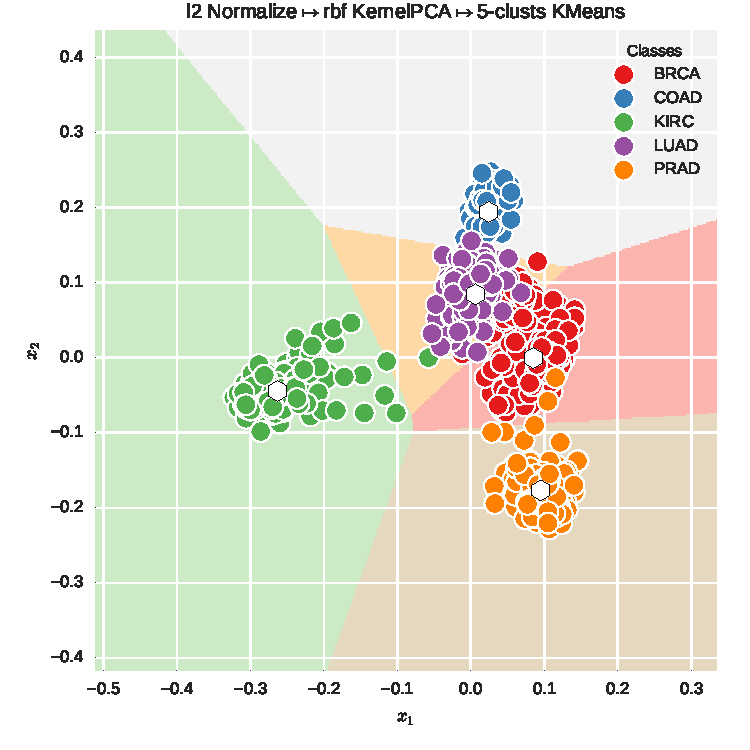
\includegraphics[width=0.4\textwidth]{figures/l2-kpca-KMeans_5-clusts.pdf}%
        \label{fig:a}%
        }%
    \hfill%
    \subfloat[]{%
        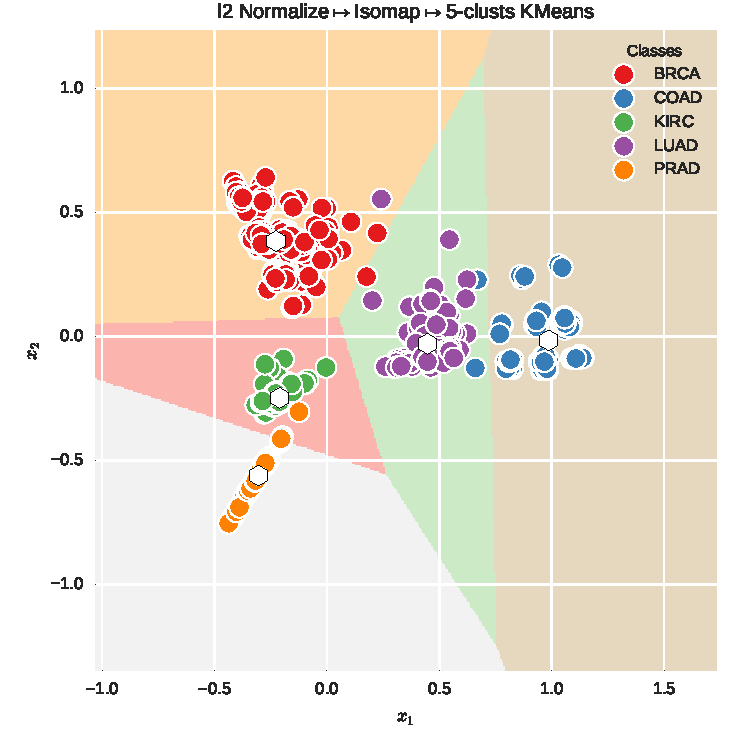
\includegraphics[width=0.4\textwidth]{figures/l2-iso-KMeans_5-clusts.pdf}%
        \label{fig:b}%
        }%
\caption{K-means performance after two different nonlinear projections. Data-points colors refer to real classes, while backgrounds are colored according to clustering predictions. The dataset is composed by a random extraction of $801$ samples (with dimension $20531$) measuring RNA-Seq gene expression of patients affected by 5 different types of tumor: breast invasive carcinoma (BRCA), kidney renal clear cell carcinoma (KIRC), colon  (COAD), lung  (LUAD) and prostate adenocarcinoma (PRAD). This reduced dataset is available from \ade documentation website and it comes from the cancer genome atlas pan-cancer analysis project~\citep{weinstein2013cancer}. In both cases our algorithm automatically discovers the correct number of clusters, even if the isomap projection improves the clustering performance.} \label{fig:scatter}
\end{figure}


% \acks{Acknowledgements go here.}

%\vskip 0.2in
\bibliography{adenine}

\end{document}
